%!TEX root = practicum1.tex
A general sketch of the situation is provided in \autoref{fig:b:leftRightTurn}. To determine whether $L$ makes a turn and in what direction we can use the angle $\theta$. Since we are not interested in the exact angle, we only need to know whether $\theta$ is zero and if not, what its sign is. 

\begin{figure}
	\centering
	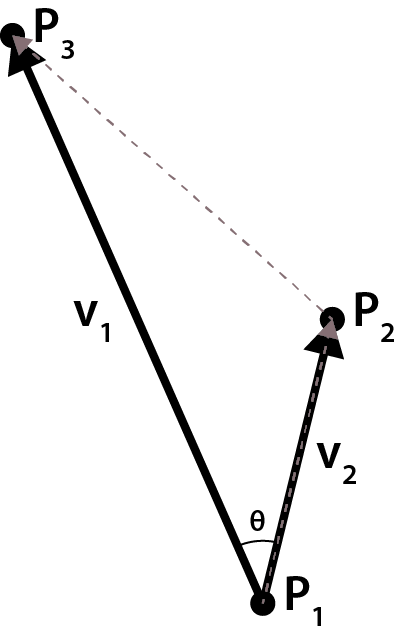
\includegraphics[scale=1]{./img/b_leftRightTurn}
	\caption{The three points $\vec{P_1}$, $\vec{P_2}$ and $\vec{P_3}$. The dashed line represents the path $L$ from point $\vec{P_1}$, through $\vec{P_2}$ to $\vec{P_3}$. $\theta$ is the angle between the vectors $\vec{v_1} = \vec{P_3} - \vec{P_1}$ and $\vec{v_2} = \vec{P_2} - \vec{P_1}$}.
	\label{fig:b:leftRightTurn}
\end{figure}

Adding a $z$-coordinate of zero to the points $\vec{P_r}$ gives us the points $\vec{P_r}'$ with $r \in \{1, 2, 3\}$. The cross product of the vectors $\vec{v_1}$ and $\vec{v_2}$ is defined as:

	\begin{equation}
		\vec{v_1} \times \vec{v_2} = \begin{pmatrix}0\\0\\q\end{pmatrix},
	\end{equation}
with $q = p1y p2x - p1x p2y - p1y p3x + p2y p3x + p1x p3y - p2x p3y$, where $p1y$ represents the second element of the point $\vec{p_1}$, the code used to derive this expression is presented in \autoref{lst:b:formalExpression}. The sign of the variable $q$ indicates what turn if any we made. If $q$ is zero there was no turn, if $q$ smaller than zero we made a right turn, if it is larger than zero a left turn.


\begin{lstlisting}[float, caption={Generation of the formal expression.}, label={lst:b:formalExpression}, language=Mathematica]
p1 = {p1x, p1y, 0};
p2 = {p2x, p2y, 0};
p3 = {p3x, p3y, 0};
v1 = p3 - p1;
v2 = p2 - p1;
Cross[v1, v2]
\end{lstlisting}



